
I would not use much time on improving integrators at this stage (the
flow is not Hamiltonian, but there is lots of literature on time-reversal
invariant dynamical systems - \refref{lamb98,LaWu02,Bosetti2010})


%unused example of t=0 line in KSe
In the time independent case, the \KSe\ on the $T=0$ line,
there is exponential growth in complexity
as space tends towards infinity\rf{Mks86}. Inclusion of time
only makes this worse; how then, can infinite space-time ever
be explained? This question is answered by the existence
of very important solutions defined on small computational domains
which we have named \textit{fundamental tiles}. This is interesting
because the dynamics on these small \spt\ domains are typically
very simple; a result of there being few invariant solutions.
It is these tiles which shall form the foundation for the
\spt\ theory.


In this report I will describe my efforts towards implementing MATLAB
code that allows for spatial integration of the \KSe. The big caveat is
that I have still not been able to accomplish this, at least as of the
time of the current version of this report.


The one spatial dimension \KSe\ is given by
\beq
    u_\zeit + u u_\conf
    + u_{\conf \conf}+\nu u_{\conf \conf \conf \conf} = 0 \,,
    \label{e-MNGre1}
\eeq
The terms of this equation all play different roles: $u_{\conf \conf}$
is an ``anti-diffusion'' term, that pumps energy into the system and
feeds instabilities on large length scales,
$u_{\conf \conf \conf \conf}$ which provides damping on small  length scales, and
the nonlinear, inertial term $u u_\conf$ which transfers energy between
large and small scales. The ``hyper-viscosity" $\nu$ plays through
the dimensionless parameter $\tildeL = L/(2\pi \sqrt{\nu})$ a role analogous
to the role that the Reynolds number $Re$ plays in the Navier-Stokes equation.

When the \KSe\ is taken with spatially periodic boundary conditions
$u(\conf + L, \zeit) = u(\conf, \zeit)$,  $u(\conf, \zeit)$
can be interpreted as  the vertical velocity
field of a ``ring of fire'', produced by a Bunsen burner, for example. A
number of studies\rf{kstroy89,kstroy92,ksgreene88,Mks86,DoLa14}
explore the steady solutions of this system, i.e., where $u_t = 0$.
These solutions are important when viewed from a topological perspective,
as the equilibria play a role in the organization of the \statesp.


In order to get into spatial integration of a time-strip, one must first generate the time strip. Because of the spatial periodicity of $u(\conf, \zeit)$, the time evolution of solutions is best done in Fourier space. The \KSe\ in Fourier space takes the form,

\beq
\dot{\tilde{u}}_k = (q_k^2-q_k^4)\utensor_k-i\frac{q_k}{2}\sum_{m=-\infty}^{\infty}\utensor_m\utensor_{k-m}
\label{e-MNGre2}
\eeq

The term with $-q_k^4$ serves to damp higher Fourier modes, which allows accurate and stable results even when truncating the infinite number of Fourier modes, a notion that makes numerical implementation feasible. Also, because $u(x,t)$ is a physical and hence, a real quantity, there also exists the relation between Fourier coefficients $u_{-k}=u_k^{*}$. Therefore for a truncation that keeps $N$ Fourier modes, we can rewrite the Fourier space equation as,

\beq
\dot{\tilde{u}}_k = (q_k^2-q_k^4)\utensor_k-i\frac{q_k}{2}\sum_{m=0}^{N/2-1}\utensor_m\utensor_{k-m}
\label{e-MNGre3}
\eeq

To integrate this equation numerically, we first start with spatially
discretizing the \KS\ system by Fourier expanding the field
$u(\conf_n,\zeit)= u_n(\zeit)$ over $N$ points of a periodic spatial
lattice $\conf_n = n L/N$,
\bea
  \utensor_k(\zeit) &=& \frac{1}{N} \sum^{N-1}_0 u_n(\zeit) e^{-iq_k\conf_n}
  \,=\, \frac{1}{N} \sum^{N-1}_0 u_n(\zeit) e^{-i 2 \pi k n /N}
  \,,\quad
q_k = \frac{2 \pi k}{L}
\continue
  u_n(\zeit) &=&\sum_{k=-N/2+1}^{N/2}\utensor_k(\zeit) e^{iq_k\conf_n}
    \,=\, \sum_{k=-N/2+1}^{N/2}\utensor_k(\zeit) e^{i 2 \pi k n /N}
\,,
\label{e-MNGre4}
\eea

where $k$ ranges from $-N/2+1$ to $N/2$ due to how MATLAB's Fast
Fourier Transform (FFT) handles an even number of configuration space points.
 In order to have a completely symmetric spectrum, one would need to have an
 odd number of configuration space points, which depending on the number and
  size of prime factors, would increase the computation time.

Following in the footsteps of others, MATLAB code \texttt{kursiv.m}
originating from Kassam and Trefethen\rf{ks05com}, is adapted in order
to provide accurate time-evolution data of $u_n(\zeit)$. The scheme used
in this implementation is a combination of two different methods,
Exponential Time Differencing (ETD) and Fourth Order Runge-Kutta (RK4)
to form a new schema aptly abbreviated ETDRK4. All of this is applied in
\texttt{ksint.m} which was written by Xiong and Ruslan. This generates the
time evolution data for spatial Fourier modes with $k = \pm 1, \pm 2, \ldots, \pm 15$.
The amplitudes for the $k=0$ and $k=-N/2$ ($N$ even), are taken to be zero.

The velocity field $u(\conf,\zeit)$ is retrieved via application of
MATLAB's Inverse Fast Fourier Transform (IFFT) on each column of
time-evolution data, which correspond to different times. The first three
spatial derivatives of the velocity field are retrieved through the
spectral method known as spectral differentiation via the equations
     \PC{2016-08-15}{Shouldn't $u_k$ be $\utensor_k$ in \refeq{e-MNGre5}?}
\bea
    u_{\conf}( \conf, \zeit) &=&
                \mathcal{F}^{-1} \left\{i q_k \utensor_k \right\} \,, \quad
    u_{\conf \conf}( \conf, \zeit) =
                \mathcal{F}^{-1} \left\{(i q_k)^2 \utensor_k \right\} \,, \quad \continue
    u_{\conf \conf \conf}( \conf, \zeit) &=&
                 \mathcal{F}^{-1} \left\{(i q_k)^3 \utensor_k \right\} \,, \quad
                 \label{e-MNGre5}
\eea
A  as we shall see in \refsect{sect:MNGspatInt}, the values of the
spatial derivatives on a time strip are required for spatial integration.

The initial conditions for the time evolution of $\PPO{10.2}$ were
provided by Xiong Ding's \texttt{ks22h02t100E.mat}.

In order to begin spatial integration, we will expand the time periodic
data generated from time integration into its discretized temporal Fourier
 modes. First we will start with the expansion of a time periodic function
 $u(\zeit) = u(\zeit + T)$, in terms of its temporal Fourier modes.

\beq
    u(\zeit) = \sum_{k = -\infty}^{\infty}
    \utensor_k e^{i \omega_k \zeit} \, , \quad \mbox{where }
    \omega_k = 2 \pi k / \period{}
\,.
\label{e-MNGre6}
\eeq

The Fourier coefficients $\utensor_k$ can be retrieved by inverting \refeq{e-MNGre6},
\beq
    \utensor_k = \frac{1}{T} \int_0^{\period{}} d\zeit\ u(\zeit)
            e^{- i \omega_k \zeit}
            \label{e-MNGre7}
\eeq

The discrete version of these relations can be obtained with the
approximation $\int_0^T dt \rightarrow \sum_{n=0}^{N-1}\Delta t$,
$\Delta t ={T}/{N} $, namely for the discrete Fourier transform,

\bea
    \utensor_k &=& \frac{1}{N} \sum_{n=0}^{N-1} u(\tn) e^{-i \omega_k \tn} \,,
    \mbox{where } \tn = n T / N \continue
          &=& \frac{1}{N} \sum_{n=0}^{N-1} u(\tn) e^{-i 2 \pi n k / N}
          \, , \continue
          &=& \frac{1}{N} \mathcal{F} \{ u (\tn) \} \, ,
\label{e-MNGre8}
\eea
and likewise for the inverse discrete Fourier transform,
\bea
    u(\tn) &=& \sum_{k = - N/2+1}^{N/2} \utensor_k
    e^{i \omega_k \tn} \, \quad \continue
               &=&\, \sum_{k = - N/2+1}^{N/2} \utensor_k e^{i 2 \pi k n / N}
\label{e-MNGre9}
\eea
The next step is to derive the form that \KSe\ takes in terms
of spatial Fourier modes. First we define,
\beq
    u^{(0)} \equiv u \, , \quad
    u^{(1)} \equiv u_{\conf} \, , \quad
    u^{(2)} \equiv u_{\conf \conf} \, , \quad
    u^{(3)} \equiv u_{\conf \conf \conf}
\label{e-MNGre10}
\eeq
which allows us to write the \KSe\ as a system of equations,
\bea
    u^{(0)}_{\conf} &=& u^{(1)} \continue
    u^{(1)}_{\conf} &=& u^{(2)} \continue
    u^{(2)}_{\conf} &=& u^{(3)} \label{e-MNGre11} \\
    u^{(3)}_{\conf} &=& - u^{(0)}_{\zeit} - u^{(2)} - u^{(0)} u^{(1)}
                        \nonumber
\,.
\eea
Now we write the equivalent expression in its Fourier representation,
taking into consideration a truncated number of Fourier modes $N$.
\bea
    \frac{\partial}{\partial \conf} \utensor^{(3)}_k &=&
        - i \omega_k \utensor^{(0)}_k
        \, - \utensor^{(2)}_k
        \, - \sum_{m = 0}^{N/2-1} \utensor^{(0)}_{m} \utensor^{(1)}_{k-m}
         \continue
    \frac{\partial}{\partial \conf} \utensor^{(2)}_{k} &=& \utensor^{(3)}_{k} \, , \continue
    \frac{\partial}{\partial \conf} \utensor^{(1)}_{k} &=& \utensor^{(2)}_{k} \, , \label{e-MNGre12} \\
    \frac{\partial}{\partial \conf} \utensor^{(0)}_{k} &=& \utensor^{(1)}_{k} \, , \nonumber
\eea
The rationale behind the truncation in this context is currently not as
solid as opposed to the time-integration of a (spatial Fourier mode
discretization). There is no longer a term in our equations that damps
the higher modes. There isn't any term that provides energy either, but
the damping was a good control of numerical accuracy. Burak has
proposed to introduce an artificial diffusion term of form $\epsilon
u_{tt}^{(3)}$ into the fourth equation in \refeq{e-MNGre11}. In the Fourier
space this would take the form $-e w_k^2 \utensor_k^{(3)}$, where $e$ is known
as an \textit{artificial diffusion constant}. In our numerics, implementing this with
$e=10^{-4}$ produced no significant effect. According to Burak, a value
$e=10^{-4}$ is still a very large value for the artificial diffusion
constant. Therefore, I did not include this term in most of my computations.

The nonlinear term can be handled in a couple of different ways. The first is to
directly calculate the convolution sum; this is undesired as it is slow and more
importantly does not treat floating-point truncation errors well. The second method
is to calculate it via pseudo-spectral method,

\beq
\sum_{m=0}^{N/2-1} \utensor^{(0)}_m \utensor^{(1)}_{k-m} = \frac{1}{N} \mathcal{F} \left\{ u^{(0)} u^{(1)} \right\} .
\label{e-MNGre13}
\eeq

The third option is to calculate it in a fully spectral manner via the circular
convolution function included in MATLAB, \texttt{cconv}. It's hard to tell which is
the best from looking at the values produced because they are all similar up to numerical
accuracy, but I would believe the pseudo-spectral method is the best because of how the
circular convolution function works, the lack of speed of the convolution sum.


An additional procedure can be applied to the pseudo-spectral method in order to
combat what is known as \textit{aliasing}. Aliasing is byproduct of discretization,
wherein the amplitude of higher frequency (or similarly high wavenumber) modes
can affect the amplitudes of lower modes. The happens when higher modes are
misrepresented as lower modes. For $k = -N/2+1, \ldots, N/2$ and  $j \in \mathcal{Z}$,

\bea
e^{\frac{i 2 \pi \left( k+jN \right) }{N}} &=& e^{\frac{i 2\pi k }{N}}*e^{i 2\pi j}\\
 &=& e^{i 2\pi k }. \nonumber
\eea

In order to account for this, one must apply a dealiasing formula to the computation
of the pseudo-spectral term. One way of accomplishing this is to zero-pad the
corresponding Fourier mode data before computing the IFFT which results in $u^{(0)}$ and $u^{(1)}$.
For example, the number of Fourier mode coefficients is increased from $N$ to $2N$
by including $N$ zero-valued coefficients. The IFFT is then applied which produces
$u^{(0)}$ and $u^{(1)}$ arrays each of length $2N$. Element wise multiplication
is used with these new arrays of length $2N$ to produce an array equal to the
product $u^{(0)} u^{(1)}$. The product is then brought back to Fourier space via FFT.
The final step is taking the new Fourier mode data, an array of $2N$ Fourier
Coefficients, and extracting the coefficients belonging to modes $k = -N/2+1, \ldots, N/2$.


\begin{figure}[ht]
\begin{minipage}[height=.45\textheight]{.45\textwidth}
\centering \small{\texttt{(a)}}
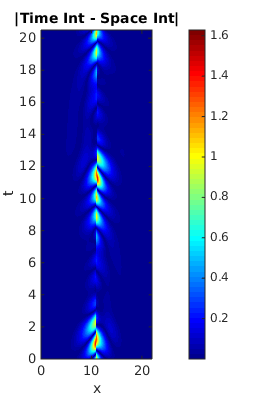
\includegraphics[width=\textwidth,height=.45\textheight]{MNGppo1m21e}
\end{minipage}
\begin{minipage}[height=.45\textheight]{.45\textwidth}
\centering \small{\texttt{(b)}}
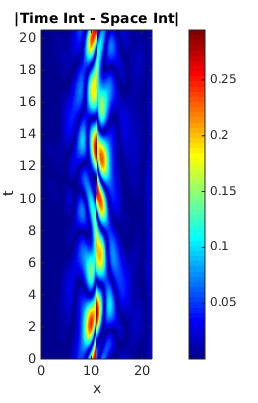
\includegraphics[width=\textwidth,height=.45\textheight]{MNGppo1m7e}
\end{minipage}
\caption{\label{fig:MNGppo1error}
Absolute error between time-integrated solutions of $\ppo{10.2}$ and spatially integrated solutions.
A Time-periodic initial condition $T = [0,2\,T_{\ppo{10.2}})$ was taken from the time integrated solution.
This initial time-strip was integrated spatially in two parts, $x = [0,11]$ and $x = [-11,0]$. The number of active Fourier modes in each plot are (a) 21, and (b) 7.
}
\end{figure}


Consider next the case of temporally periodic velocity field
\beq
    u(x, t) = u(x, t + \period{})
\label{e-PeriodicBC}
\eeq
on temporal domain of fixed period $\period{}$,
and any x, \ie, cylinder $(x,t) \in \reals \times [0,\period{})$, see
\reffig{fig:spaceTime1}\,(b).

In order to express
\KS\ as a set of first-order PDEs, define four fields
\beq
(u_{0},u_{1},u_{2},u_{3}) \equiv
(u,
u_{x},
u_{x x},
u_{x x x})
\,.
\eeq
Using the values of the four fields
for all $t \in [0, \period{})$ at a fixed space point $x_0$,
as initial values,
one may attempt
to determine $u(t, x)$ for any $x$ on a time-periodic strip
$t \in [0, \period{})$ by solving the \KS\ \refeq{e-ks}
rewritten as a set of equations first order in spatial
derivatives
    \PC{2016-07-23}{The equations seem correct to me.
    The notation of \refrefs{LanThesis,lanCvit07} is different, but
    Burak's $u^{(j)}$ fields are easier to keep track of.
    {\bf 2019-05-18 PC} experimenting with $u_j$ format.
    }
\bea
    \frac{\partial}{\partial x} u_{0} &=& u_{1} \,,\quad
    \frac{\partial}{\partial x} u_{1} \,=\, u_{2} \,,\quad
    \frac{\partial}{\partial x} u_{2} \,=\, u_{3} \,, \label{e-ksX} \\
    \frac{\partial}{\partial x} u_{3} &=&
    - \frac{\partial}{\partial t} u_{0} - u_{2} - u_{0} u_{1}
\nonumber
\,.
\eea
Given the time-periodic boundary condition \refeq{e-PeriodicBC},
it is natural to expand the \KS\ field $u(x,\tn)= u_n(x)$ as a temporal Fourier
$u(x,\tn)= u_n(x)$ over $M$ points of a periodic
temporal lattice $\tn = n \period{}/M$, $n=0,1,\cdots,M-1$:
\beq
    u_{i}(x, t) = \sum_{n = 0}^{M-1}
    \utensor_{i,n}(x)\,e^{i \omega_n \tn} \, , \quad \mbox{where }
    \omega_n = 2 \pi n / \period{} \, .
\ee{BBtemporFourier}
Rewriting \refeq{e-ksX} in terms of temporal Fourier modes,
we obtain $4M$ ordinary differential equations,
\bea
\frac{\partial}{\partial x} \utensor_{0,n} &=& \utensor_{1,n}
         \continue
\frac{\partial}{\partial x} \utensor_{1,n} &=& \utensor_{2,n}
        \continue
\frac{\partial}{\partial x} \utensor_{2,n} &=& \utensor_{3,n}
        \label{e-FksX} \\
\frac{\partial}{\partial x} \utensor_{3,n}
      &=&
 - i \omega_n \utensor_{0,n} - \utensor_{2,n}
 - \sum_{n' = 0}^{M-1} \utensor_{0,n - n'} \utensor_{1,n'}
\,. \nonumber
\eea
%Due to their instabilities, these equations might
%be hard to integrate numerically.
    \PC{2016-09-12, 2016-09-23}{Checked, except for the range of $n'$.}

\subsubsection{Integrating \KS\ on a $\period{}=0$ line}
\label{sect:KSeqva}

%     BB 2016-02-04, PC 2016-09-23
If $u$ is a temporal \eqv, $u = u(x+vt,0)$ whose spatial profile
does not change in time, with a vanishing $u_t=0$ (for an \eqv) or a constant
traveling wave velocity $u_t=v$ (for a \reqv), one can integrate \refeq{e-ks}
\beq
    u_t -v = 0
    = - \left(u^2/2 -u_{x}-u_{x x x}\right)_{x}
\label{e-ksSteady}
\eeq
once over space, and the highest order derivative in \refeq{e-ksX}
becomes the third order\rf{Mks86,LanThesis,lanCvit07,DoLa14}. We shall
refer to this case as the $\period{}=0$ temporal strip, as specifying $u
= u(x_0,0)$ at $t=0$ instant suffices to initialize the spatial
evolution, which in this case is given by a set of three ODEs and an
integration constant, which can be interpreted as the energy density $\expctE$,
\beq
\expctE = {\textstyle\frac{1}{2}}u^2 - c u + u_x + u_{xxx}
\,.
\label{SCD07eq:stdks}
\eeq
% \PCpost{2018-05-30}{
Computationally, it is more robust to compute $\expctE$ by averaging over $\speriod{}$,
as in \refeq{SCD07ksEnergy}.

Eqs.~\refeq{e-ksX}, however, remain a set of four PDEs for any
$\period{}>0$ temporal strip.

\subsubsection{Spatial stability of $u=0$ equilibrium}
\label{sect:KSu0equiS}

To calculate the spatial stability of a spatial \eqv, we need to evaluate
the \stabmat\ of the system in the complex representation \refeq{e-FksX}
in terms of the 16 sub-blocks
\beq
  \Mvar_{ij}^{IJ} (\utensor)  =
\frac{\partial \utensor^{'}{}^{(I)}_i}
     {\partial \utensor{}^{(J)}_j}
\,,\qquad
    \utensor^{'} = \utensor_x
\,.
\ee{eq:StabMatBlocks}
The trivial \eqv\ of \refeq{e-FksX} is given by $\utensor^{(I)}_{j}=0$.
In terms of $[M\!\times\!M]$ temporal Fourier modes blocks its spatial
\stabmat\ is
\beq
\Mvar^{IJ}(0) =
\begin{bmatrix}
  0 & 1 & 0 & 0 \\
  0 & 0 & 1 & 0 \\
  0 & 0 & 0 & 1 \\
\mbox{Diag}\{-i \omega_k\} & 0 & -1 & 0
\end{bmatrix}
\ee{PCeqvaStblty}


The actual implementation concerning the integration of these equations was to use the
MATLAB's stiff-ODE integrator \texttt{ode15s}. This integrator has higher accuracy than
some of its counterparts, such as \texttt{ode23s} and \texttt{ode23tb}. The integrator is
designed to be used with its own variable step size algorithms in order to deal with the
stiffness of equations, however, linearly space steps can be used if so desired. The error
 tolerances can also be controlled using \texttt{ode15s} while using a variable step size.

so that the relative tolerance is much more useful when dealing with small numbers. If the
 relative tolerance is set to be too low, accumulated round off errors will dominate the
 inaccuracy, while if it is set too high the local discretization errors will dominate.

The integrator requires a separate MATLAB file, \texttt{velocityfunction.m} whose
input is $\utensor^{(i)}_{k}$, for $i = 0,1,2,3$ according to \refeq{e-MNGre10} and whose
 output is $\frac{\partial}{\partial \conf}\utensor^{(i)}_{k}$ i.e. it is the implementation of \refeq{e-MNGre12}.

Once the integrator has finished running, my current MATLAB code
\\
\texttt{timeperiodic.m} converts the spatial evolution of the Fourier
coefficients $\utensor_k^{(i)}$ $i = 0,1,2,3$ into the four (discretized)
spatial fields $(u,
u_\conf, u_{\conf \conf}, u_{\conf \conf \conf})$ via the use of
MATLAB's IFFT.

\subsubsection{Spatial integration results}
In its current form, my code is only able to give somewhat sensible
results for short spatial integrations $\conf = [0, L]$, $L = \approx 1$,
where the period of the desired spatially periodic solution is known to
be $L=22$.

This can be seen by looking at the Fourier coefficient amplitudes over
the course of spatial integration, see \reffig{fig:MNGrfig1}. The spectrum
seems to flatten, i.e. the amplitudes of the higher modes grow
dramatically as the spatial extent of the integration is increased.

Considering these limitations I work around the fact that there is a
limited spatial extent on which my integrator seems to work. The way that
I decided to deploy my code was the take increase the number of
configuration space points to 64 in order to increase the resolution and
then integrate the 64 corresponding time-periodic strips over $x = [0,
22/64] = [0, 0.34375]$. I then combine the results such that the
resulting figure attempts to represent spatial integration for $x =
[0,22]$. This technique is not able to exploit the variable step size of
the integrator, as the strips would be of varying sizes and hence the
compilation would not be a very meaningful visualization.

\begin{figure}[h]
  \begin{minipage}[height=.40\textheight]{.35\textwidth}
    \centering \small{\texttt{(a)}}
    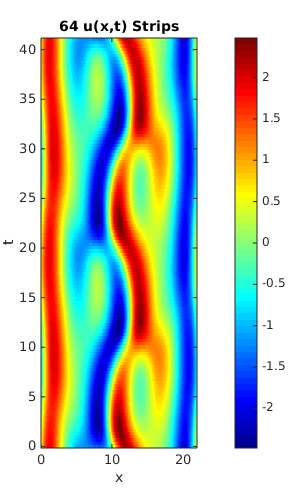
\includegraphics[width=\textwidth,height=.45\textheight]{MNGcompxint22}
  \end{minipage}
  \begin{minipage}[height=.40\textheight]{.35\textwidth}
    \centering \small{\texttt{(b)}}
    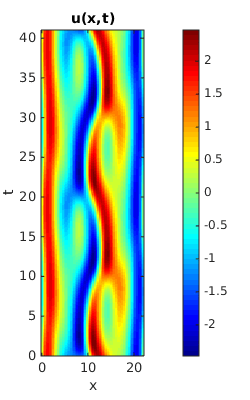
\includegraphics[width=\textwidth,height=.45\textheight]{MNGppo1timeint}
  \end{minipage}
   \caption{Comparison of (a)compilation of 64 spatial integration strips integrated over $x=[0,0.34375]$ and (b) time integration of \PPO{10.2} integrated over time $T = [0,4\,T_{\PPO{10.2}}$, for system size $L=22$}
  \label{fig:MNGrfig2}
\end{figure}

The \reffig{fig:MNGrfig2} is a comparison between the spatial integration
of \refeq{e-MNGre12} using the compilation method I employed in
\texttt{timeperiodic.m} and the time integration of \refeq{e-MNGre3}
using the ETDRK4 numerical scheme implementation of MATLAB file
\texttt{ksint.m}. The behavior of these figures seem to exhibit similar
patterns up to a what appears to be a reflection in the time direction,
implying that there is some unaccounted symmetry. This can be seen by
what I call the ``tails" of the pattern in the middle being pointed in
opposite directions for time and space integration.

The hope for my code is to be capable of spatial integration of infinite
 extent. My results are disappointing to me to say the least, having been
  thrown for loops by what should have been insignificant details, but
  I hope to use what I've learned in terms of coding in the future.

Some possible means of improving the equations is to look for better ways to
 dealias the pseudo-spectral term or to use the same method but require it to be more rigorous (e.g. more zero-padding).

Second would be to write an integration scheme that could produce more
accurate results. My first thought is to apply the ETDRK4 schema to spatial
 integration, however, I'm not sure if this would work with a system of
 equations rather than a single PDE.

